\section{Random Variables}
\label{sec:random_variables}
A \textbf{random variable}, $\tilde{x}$, is a mathematical representation of a value and its associated uncertainty. Usually, we are interested not just in the behaviour of a certain value of a variable or parameter, but also in how it behaves when it is uncertain. A \textit{sample} of such random variable can take several values according some \textbf{distribution law}. So we are specially interested in how this distribution law \textit{reshapes} when passing through different physical processes and/or computation steps. The \textbf{probability density function}, also known as PDF, or just \textit{density}, is a function 
\begin{equation}
F_{\tilde{x}}(x):\mathbb{R}\rightarrow \mathbb{R} 
\end{equation}
that expresses which values in the domain of the variable $x$ are more likely, according to the random variable $\tilde{x}$. However, since this function is a density, the actual value expressing a probability is the integral between an interval:
\begin{equation}
p(a<\tilde{x}<b) = \int^b_a F_{\tilde{x}}(x) dx 
\end{equation}

A \textbf{random vector}, $\tilde{\mathbf{x}}$, is an array of random variables, stacked forming a column vector: 
\begin{equation}
\tilde{\mathbf{x}} =
\left[
\begin{array}{c}
 \tilde{x}_1\\
 \tilde{x}_2\\
 \vdots \\
 \tilde{x}_n\\
\end{array}
\right].
\end{equation}
In such case, the probability density function is defined as: 
\begin{equation}
F_{\tilde{\mathbf{x}}}(\mathbf{x}):\mathbb{R}^n\rightarrow \mathbb{R} 
\end{equation}
and the probability in a given interval,~$I$, is computed as:
\begin{equation}
p(\tilde{\mathbf{x}}\in I) = 
p(a_n<\tilde{x}_1<b_n,\dots,a_n<\tilde{x}_n<b_n) = 
\int^{b_1}_{a_1} \dots \int^{b_n}_{a_n} F_{\tilde{\mathbf{x}}}(\mathbf{x}) dx_n \dots dx_1 
\end{equation}

\subsection{Moments}
A way to parameterize a distribution law is through its \textit{moments}, a set of parameters that can fully describe the distribution in some cases, or just approximate it in others. The most known moments are the mean, $\mu$, which is the fisrt order moment, and the variance, $\sigma^2$, which is the second order moment.

In the unidimensional case, from a set of $p$ samples $\{x_1\dots x_p\}$, $x_i \in\mathbb{R}$, the mean and variance can be estimated as:
\begin{equation}
 \mu_x = \frac{1}{p}\sum^p_{k=1} x_k;\ \ \ \sigma^2_x = \frac{1}{p-1}\sum^p_{k=1} (x_k-\mu_x)^2;
\end{equation}

In the multivariate case the mean becomes a vector, $\boldsymbol\mu_x\in\mathbb{R}^n$. Given~$p$ samples, it can be estimated as:
\begin{equation}
 \boldsymbol\mu_x = \frac{1}{p}\sum^p_{k=1} \mathbf{x}_k;
\end{equation}
In that multivariate case, the second order moment can be \textit{cross}computed, so a \textit{covariance} matrix is used to describe the second order stathistics, which has the following squared form: 
\begin{equation}
 \mathbf{C}_x = 
 \left[
 \begin{array}{cccccc}
  c_{11} & \dots & \dots & c_{1j} & \dots & c_{1n} \\
  \vdots &       &       & \vdots &       & \vdots \\
  c_{i1} & \dots & \dots & c_{ij} & \dots & c_{in} \\
  \vdots &       &       & \vdots &       & \vdots \\
  c_{n1} & \dots & \dots & c_{nj} & \dots & c_{nn} \\
 \end{array}
 \right];
\end{equation}
From a set of~$p$ samples, the element $c_{ij}$ of the covariance matrix is estimated as follows: 
\begin{equation}
 c_{ij} = \frac{1}{p-1}\ (\mathbf{s}_{x_i}-\mu_{x_i})^T \cdot (\mathbf{s}_{x_j}-\mu_{x_j})
\end{equation}
where $\mathbf{s}_{x_i}$ is a vector stacking all $p$ samples of component~$i$ of the random variable~$\tilde{\mathbf{x}}$, and a subtracting a scalar from a vector means that we substract the scalar at all components of the vector. 

\paragraph{Interpretation of Covariance Matrix}
Recalling the interpretation of the scalar product as a measure of similarity between two vectors (subsection~\ref{subsec:norm_dot_cross}), the element $c_{ij}$ of a covariance matrix is encoding the alignment between the components~$i$ and~$j$ of the random variable~$\tilde{\mathbf{x}}$ in the set of~$p$ samples, once the mean is subtracted. Two components that suffer from the similar variations in the sample set, will appear as two vectors~$\mathbf{s}_{x_i}$ and~$\mathbf{s}_{x_j}$ nearly aligned, so its covariance~$c_{ij}$ will be close to $\frac{1}{p-1}$. In contrast, two components of the random variable~$\tilde{\mathbf{x}}$ that change without any relation, lead to two vectors~$\mathbf{s}_{x_i}$ and~$\mathbf{s}_{x_j}$ unaligned, so the scalar product, and thus the $c_{ij}$, will approach to~$0$.

So, the covariance matrix builds a base of $n$ vectors (not necessarily orthogonal!) in the space of the random variable~$\tilde{\mathbf{x}}$ with directions according how individual components behave similarly or not in the dataset of~$p$ samples. SVD decomposition can be applied to find out the main orthogonal directions of this base. 

\paragraph{Example \theexamplecounter. Compute a 2D covariance matrix from data [Scilab].}
\stepcounter{examplecounter}
In this example we'll generate two sample sets $S_1$ and $S_2$, each one composed by $100$ samples in~$\mathbb{R}^2$, so $100$ points $(x,y)$. $S_1$~is built forcing a strong linear relation between first and second component, while~$S_2$ is just computed by drawing random values for both components. The code below computes the covariance matrix for both sets.
\begin{mdframed}
\tiny
\begin{verbatim} 
//user entries
mm = 0.3;
bb = 0;
noise_stdev = 0.3; //sqrt(noise_variance)

//create set S1
xx1 = [0:0.1:10]';
[nn cols] = size(xx1); //get set size
yy1 = mm*xx1 + bb + noise_stdev*rand(nn,1,"normal");

//create set S2
xx2 = noise_stdev*rand(nn,1,"normal");
yy2 = noise_stdev*rand(nn,1,"normal");

//compute means, each component, each set:
mx1 = sum(xx1)/nn;
my1 = sum(yy1)/nn;
mx2 = sum(xx2)/nn;
my2 = sum(yy2)/nn;

//compute covariance matrix explicitly
cxx1 = (xx1-mx1)'*(xx1-mx1)/(nn-1);
cyy1 = (yy1-my1)'*(yy1-my1)/(nn-1);
cxy1 = (xx1-mx1)'*(yy1-my1)/(nn-1);
cxx2 = (xx2-mx2)'*(xx2-mx2)/(nn-1);
cyy2 = (yy2-my2)'*(yy2-my2)/(nn-1);
cxy2 = (xx2-mx2)'*(yy2-my2)/(nn-1);

//compute covariance matrix with scilab call
C1 = cov(xx1,yy1);
C2 = cov(xx2,yy2);
\end{verbatim} 
\end{mdframed}
The resulting covariance matrices are:
\begin{equation}
\small
\mathbf{C}_1 = 
\left[
 \begin{array}{cc}
    8.585      &  2.6312156  \\
    2.6312156  &  0.8963398  \\
 \end{array}
 \right];\ \ 
\mathbf{C}_2 = 
\left[
 \begin{array}{cc}
    0.0930911  & - 0.0006647  \\
  - 0.0006647  &  0.0884355   \\
 \end{array}
 \right];\ \ 
\end{equation}
The resulting matrices show how the set $S_1$ presents a much higher relation between~$x$ and~$y$ components than~$S_2$, due to the linear relation imposed when building the sets. Moreover, the fact that the values in~$C_1$ are much larger is caused because~$S_1$ stretches in the $XY$ plane occupying a larger region than~$S_2$.

\paragraph{Example \theexamplecounter. Ellipses from a 2D covariance matrix.}
\stepcounter{examplecounter}
This example shows a Scilab function to draw a 2D ellipses from a covariance matrix, centered at a given $(x,y)$ point. Numerical errors can lead to non-positive-definite covariance matrixes after some computational steps. Therefore, the first calls in the function are related to ensure that the matrix is strictly positive-definite, a necessary condition to assure eigenvalues are real (TBC!!). Positive-definite is ensured through a Cholesky decomposition. Thereafter, eigenvalues are computed, which directly provide the length of a major and minor axes of the ellipses. Finally, drawing is performed point by point over the ellipses, with steps of $0.1$ radian. 
\begin{mdframed}
\tiny
\begin{verbatim} 
//covariance matrix Cmat, and centered at point mu
function[] = draw_ellispes_from_cov(mu, Cmat, axes_h)

    //ensure positive-definite matrix
    Cchol = chol(Cmat);
    CC = Cchol'*Cchol;  
    
    //compute eigenvalues
    [RR,diagCC] = spec(CC);
    eval1 = diagCC(1,1);
    eval2 = diagCC(2,2);
    
    //sort evals by value. Set major and minor axes.
    if (eval1>eval2) then
        axis = [eval1;eval2;atan(RR(2,1)];
    else
        axis = [eval2;eval1;atan(RR(2,2)];
    end

    //start drawing (compute all points) 
    step = 0.1; //Set drawing step    
    t = 0:step:%pi/2; //set drawing vector
    eX = axis(1)*cos(t); //ellispes points (X component, a quarter)
    eY = axis(2)*sin(t); //ellipses points (Y component, a quarter)
    nn = 4*size(eX,'*'); //num of total points of the ellipses
    eXY1 = [eX, -flipdim(eX,2), -eX, flipdim(eX,2); eY, flipdim(eY,2), -eY, -flipdim(eY,2)];
    eXY = rotate(eXY1, axis(3)) + [mu(1)*ones(1,nn);mu(2)*ones(1,nn)];
    sca(axes_h); //Set current axes
    xpoly(eXY(1,:), eXY(2,:));

endfunction
\end{verbatim} 
\end{mdframed}




% \paragraph{Example \theexamplecounter. Bounding box from a set of 2D points.}
% \stepcounter{examplecounter}


% \subsection{Higher order moments}
% Third and fourth order moments are called skewness and kurtosis.  

\subsection{Uniform distribution}
A random variable or vector is called uniform when the density is constant over a bounded interval, meaning that the variable is equally distributed within this interval. That implies also that the variable can take, with equal probability, values within this interval. 

Uniform random variables can be described with just two parameters: $x_{min}, x_{max}$. The mean and the variance values of an unfiorm random variable are:
\begin{equation}
 \mu_{\tilde{x}} = \frac{x_{min}+x_{max}}{2}; \ \ \sigma^2_{\tilde{x}} = \frac{1}{12}(x_{max}-x_{min})^2
\end{equation}
%TODO: Example of C++/std code for uniform random generator}

\subsection{Gaussian distribution}
A random variable is called Gaussian or Normal, when its density is fully described with two parameters, $\mu_{\tilde{x}}$ (mean) and $\sigma^2_{\tilde{x}}$ (standard deviation), and the following expression:
\begin{equation}
 F_{\tilde{x}}(x) = \frac{1}{2\pi}e^{-(\frac{x-\mu_{\tilde{x}}}{\sigma_{\tilde{x}}})^2}
\end{equation}
Gaussian variables are also written as $\mathcal{N}(\mu,\sigma)$, which is a widely used notation stressing the dependency with just two parameters. Given $\tilde{x}=\mathcal{N}(\mu_x,\sigma_x)$ and $\tilde{y}=\mathcal{N}(\mu_y,\sigma_y)$, the following properties fulfill:
\begin{itemize}
 \item $\tilde{z}=a\tilde{x} \ \rightarrow \tilde{z}=\mathcal{N}(a\mu_x,a\sigma_x)$
 \item $\tilde{z}=\tilde{x}+\tilde{y} \ \rightarrow \tilde{z}=\mathcal{N}(\mu_x+\mu_y,\sqrt{\sigma^2_x+\sigma^2_y})$
\end{itemize}
The two properties listed above are of major importance since they imply that we know how Gaussian variables behave when they pass through linear systems. 
%example code for normal random generator and then computation of mean and variance

\subsection{Multivariate Gaussian distribution}
\label{subsec:mulivariate_gaussian_distribution}
In case of $n$-dimensional Gaussian variables, the mean is $\boldsymbol{\mu} \in \mathbb{R}^n$, and the covariance is represented as a squared matrix, $\mathbf{C}\in\mathbb{R}^{n\times n}$. The generalized formula is the following: 
\begin{equation}
 F_{\tilde{x}}(\mathbf{x}) = \frac{1}{\sqrt{\vert \mathbf{C}\vert}(2\pi)^n}
			    e^{-\frac{1}{2}(\mathbf{x}-\boldsymbol\mu)^T\mathbf{C}^{-1}(\mathbf{x}-\boldsymbol\mu)}
\end{equation}
\begin{figure}[bth!]
  \begin{center}
    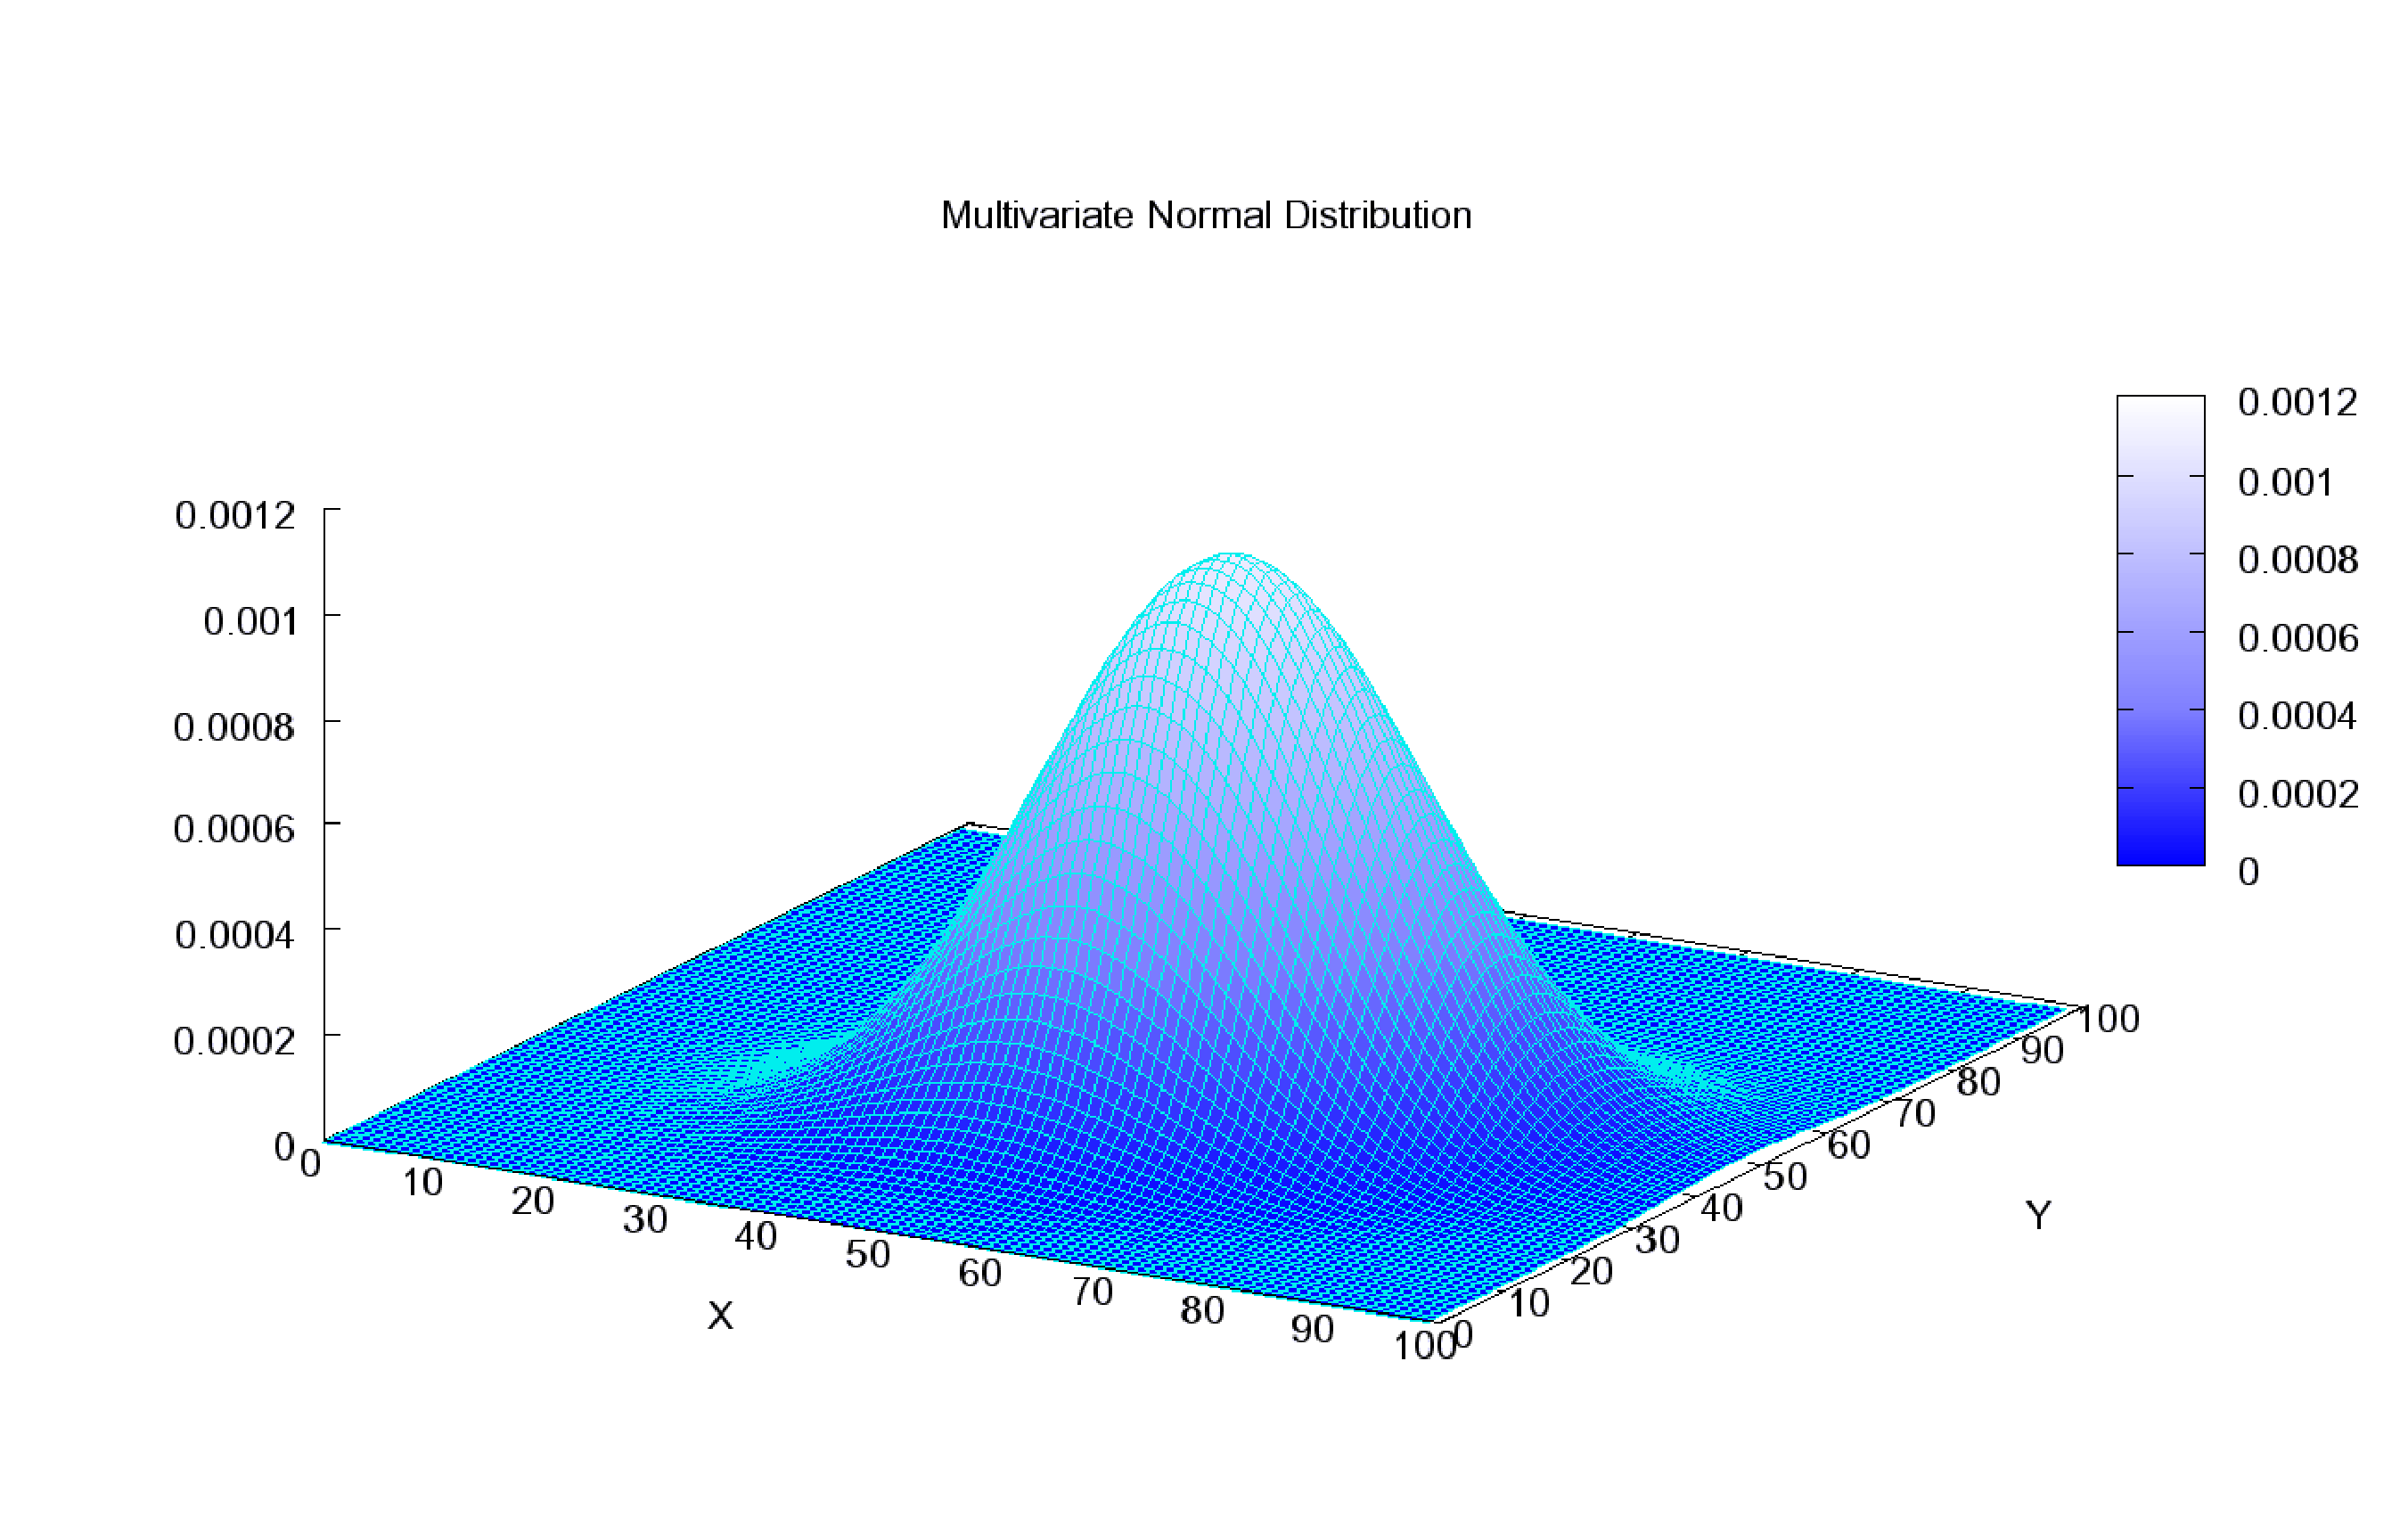
\includegraphics[width=1.0\columnwidth]{figures/mv_gaussian.eps}
    \caption{Bivariate Gaussian function}
    \label{fig:mv_gaussian}
  \end{center}
\end{figure}

In the multivariate case, the properties around the sum and the linear operation also fulfill: 
\begin{itemize}
 \item $\tilde{\mathbf{z}}=\mathbf{A}\tilde{\mathbf{x}} \ 
      \rightarrow \tilde{\mathbf{z}}=\mathcal{N}(\mathbf{A}\boldsymbol\mu_x,\mathbf{A}\mathbf{C}_x\mathbf{A}^T)$, 
      where $\mathbf{A}\in \mathbb{R}^{m \times n}$.
 \item $\tilde{z}=\tilde{x}+\tilde{y} \ 
      \rightarrow \tilde{z}=\mathcal{N}(\mu_x+\mu_y,\sqrt{\sigma^2_x+\sigma^2_y})$
\end{itemize}


\subsection{Gaussian Uncertainty Propagation}
How uncertainty is propagated through different physical or computing processes is a major topic in robotics, specially in perception, but also in precise actuation. Specifically, we are interested in know how a density function reshapes due to some computation, view point change, ...

In previous subsections we've seen that Gaussian random variables and vectors have the great property that it is easy (not only conceptually but also computationally) to compute their parameters once they pass through linear operations (product by scalar and sum). We've also seen in section~\ref{sec:Linearization} that non-linear functions can be linearized, by assuming a linearization error. Therefore, linearization and Gaussian uncertainty propagation are two operations very common in many robotics algorithms. At intuitive level, linearization remains valid as long as uncertainty is enough \textit{small} with respect to how the function changes (indicated by Jacobian). 

\paragraph{Example \theexamplecounter. Vehicle frames revisited (with uncertainty)}
\stepcounter{examplecounter}
Let's come back to the example presented in subsection~\ref{subsec:homogeneous_matrix}. However, now we will focus only in the system vehicle-sensor-point, but we will introduce two uncertainty sources: sensor measurement noise and sensor mounting point innacuracies (which can be also called extrinsics calibration uncertainty).  

First of all, the point~$\mathbf{q}$ is reported by a sensor in polar coordinates $(q_r,q_{\alpha})$. The datasheet of that sensor indicates standard deviations for range measurement and azimuth~$\sigma_r$ and~$\sigma_{\alpha}$ respectively. So the covariance matrix of a point~$q$ at the measurement space $(r,\alpha)$ is:
\begin{equation}
 \mathbf{C}_{q^{r\alpha}} = 
 \left[
 \begin{array}{cc}
 \sigma^2_r & 0                \\
 0          & \sigma^2_{\alpha} \\
 \end{array}
 \right]
\end{equation}
Point~$\mathbf{q}$ in the 2D-cartesian space, with respect to the sensor frame, is computed as:
\begin{equation}
\mathbf{q}^S\\
=
 \left[
 \begin{array}{c}
 q^S_x \\
 q^S_y
 \end{array}
 \right]
  =
 \left[
 \begin{array}{c}
 q_r \cos (q_\alpha) \\
 q_r \sin (q_\alpha) \\
 \end{array}
 \right]
\end{equation}
The equation above is not linear in the random variables, $[q_r, q_\alpha]^T$, so to propagate the uncertainty from the measurement space $(r,\alpha)$, to the 2D-cartesian one $(x,y)$, we have to linearize this equation. From the section~\ref{sec:Linearization}, we learned that multivariate functions require to compute the Jacobian in order to linearize the function around a point of interest, $(q_r,q_{\alpha})$:
\begin{equation}
 \mathbf{J}^{\mathbf{q}^S}_{r\alpha} = 
 \left[
 \begin{array}{cc}
 \cos (q_\alpha)  & -q_r\sin (q_\alpha) \\
 \sin (q_\alpha)  &  q_r\cos (q_\alpha) \\
 \end{array}
 \right]
\end{equation}
Once we know the (approximative) linear relation between~$\mathbf{q}^S$ and~$\mathbf{q}^{r\alpha}$, we can propagate the uncertainty from the polar $(r,\alpha)$ space to the 2D-cartesian $(x,y)$ space, by using the properties of how Gaussian ranodm variables modify through linear systems, as discussed in subsection~\ref{subsec:mulivariate_gaussian_distribution}:
\begin{equation}
 \mathbf{C}_{\mathbf{q}^S} = \mathbf{J}^{\mathbf{q}^S}_{r\alpha}\mathbf{C}_{\mathbf{q}^{r\alpha}} (\mathbf{J}^{\mathbf{q}^S}_{r\alpha})^T
\end{equation}
where the Jacobian has to be evaluated at the point~$(q_r,q_{\alpha})$.

At this point we have propagated the the uncertainty of the point measurement in sensor frame from the polar space to the 2D-cartesian space. But we want to compute the uncertainty of the point~$\mathbf{q}$ with respect to the vehicle frame. According to the example of vehicle frames, the expression of $\mathbf{q}^B$ is: 
\begin{equation}
\label{eq:qB_expression}
\left[
\begin{array}{c}
    \mathbf{q}^B\\
    1 \\
 \end{array}
\right] = 
 \left[
 \begin{array}{ccc}
  \cos\beta & -\sin\beta & m^B_x \\
  \sin\beta & \cos\beta & m^B_y \\
  0 & 0 & 1
 \end{array}
 \right]
 \left[
 \begin{array}{c}
  q^S_x \\
  q^S_y \\
  1
 \end{array}
 \right]
 = 
 \left[
 \begin{array}{c}
  q^S_x\cos\beta - q^S_y\sin\beta + m^B_x \\
  q^S_x\sin\beta + q^S_y\cos\beta + m^B_y \\
  1
 \end{array}
 \right]
\end{equation}
which depends on 5 uncertain variables: $(q^S_x, q^S_y, m^B_x, m^B_y, \beta)$. Again, the relation is not liinear with all the involved variables, so it is required to compute the Jacobian of the above expression, in  order to propagate uncertainty from the involved variables to the final resulting point $\mathbf{q}^B$. This Jacobian, $\mathbf{J}_{q^S,m^B,\beta}$, a $2\times 5$ matrix:
\begin{equation}
 \mathbf{J}_{q^S,m^B,\beta} = 
 \left[
 \begin{array}{ccccc}
 \cos \beta & -\sin \beta & 1 & 0 & -q^S_x\sin\beta - q^S_y\cos\beta  \\
 \sin \beta & \cos \beta & 0 & 1 &  q^S_x\cos\beta - q^S_y\sin\beta \\
 \end{array}
 \right]
 \end{equation}

Covariance matrix related to $(q^S_x, q^S_y)$ is $\mathbf{C}_{\mathbf{q}^S}$, and was computed previously. Uncertainty of the sensor mounting point is represented with the covariance matrix related to $(m^B_x, m^B_y, \beta)$: 
\begin{equation}
 \mathbf{C}_{m^B,\beta} = 
 \left[
 \begin{array}{ccc}
 \sigma^2_{m_x} & 0 & 0  \\
 0 & \sigma^2_{m_y} & 0 \\
 0 & 0 & \sigma^2_{\beta} \\
 \end{array}
 \right]
\end{equation}
So the final covariance matrix of the point $\mathbf{q}$, with respect to the vehicle frame, $\mathbf{q}^B$, is: 
\begin{equation}
 \mathbf{C}_{\mathbf{q^B}} = 
 \mathbf{J}_{q^S,m^B,\beta}
 \left[
 \begin{array}{cc}
 \mathbf{C}_{\mathbf{q}^S} & \left[0\right]_{2\times 3} \\
 \left[0\right]_{3\times 2} & \mathbf{C}_{m^B,\beta} \\
 \end{array}
 \right]
 \mathbf{J}_{q^S,m^B,\beta}^T
\end{equation}

The SciLab code below implements all this example and plots the ellispes related to~$\mathbf{C^S_q}$ and~$\mathbf{C^B_q}$.
\begin{mdframed}
\tiny
\begin{verbatim} 
 //clear
clear;

//include files (where draw_ellispes_from_cov() function is defined)
exec("/home/andreu/dev/uncertainty_propagation/ellipsesAxis.sci");

//Sensor point q detection in polar coordinates (r,a) (measurement space)
r_q = 8;
a_q = 23*%pi/180; //rad  (20.467)
qS = [r_q*cos(a_q); r_q*sin(a_q);1]; //point q in homogeneous coordinates wrt to the Sensor

//sensor noise in polar coordinates (measurement space) 
sigma_range = 0.03; //meters 
sigma_angle = 0.1*%pi/180; //rad 
Cra_q = [sigma_range^2 0;0 sigma_angle^2]; //covariance matrix in measurement space
J_ra = [cos(a_q) -r_q*sin(a_q); sin(a_q) r_q*cos(a_q); 0 0]; //Jacobian: Linearization from measurement to homogeneous space

//Sensor mounting point with respect to the vehicle base
betaB_S = 35*%pi/180; //orientation angle of the sensor wrt the base
mB_S = [31;12]; //xy coordinates of the sensor wrt the base
RB_S = [cos(betaB_S) -sin(betaB_S); sin(betaB_S) cos(betaB_S)]; //rotation of the sensor wrt the base (R base2sensor)
TB_S = [RB_S mB_S;0 0 1]; //homogeneous transform of the sensor wrt the base (T base2sensor)

//sensor mounting point uncertainty (calibration error, or on-line sensor frame positioning error)
sigma_mx = 0.005; //meters
sigma_my = 0.005; //meters
sigma_beta = 0.1*%pi/180; //rad
C_mbeta = [sigma_mx^2 0 0; 0 sigma_my^2 0; 0 0 sigma_beta^2];
J_mbeta = [1 0 -qS(1)*sin(betaB_S)-qS(2)*cos(betaB_S); 0 1 qS(1)*cos(betaB_S)-qS(2)*sin(betaB_S); 0 0 0];

//------------------ PROPAGATE COVARIANCES --------------
CS_q = J_ra*Cra_q*J_ra'; disp(CS_q);
CB_q = TB_S*CS_q*TB_S' + J_mbeta*C_mbeta*J_mbeta'; disp(CB_q);

//------------------- DRAW ELLIPSES ---------------------
figure('BackgroundColor',[1 1 1]);
drawaxis();
ph = gca(); // handle
ph.isoview = 'on';
ph.axes_visible = ["on","on","off"]
ph.grid = [1,1];
ph.auto_scale="on";
ph.auto_clear = 'off';

//CS_q
draw_ellispes_from_cov([0 0], CS_q(1:2,1:2),ph);
e=gce(); // get the current entity (the last created, the ellipses)
set(e,"foreground",1);
set(e,"thickness",3);
ph.auto_clear = 'off';

//CB_q
draw_ellispes_from_cov([0 0], CB_q(1:2,1:2),ph);
e=gce(); // get the current entity (the last created, the ellipses)
set(e,"foreground",2);
set(e,"thickness",3);
\end{verbatim}
\end{mdframed}
For the values of the code example above, the two plotted ellipses are shown in Figure~\ref{fig:ellipses}. In the black ellispes related to the point uncertainty with respect to the sensor frame,~$\mathbf{C^S_q}$, it can be seen how the shape of the uncertainty is larger in the range measurement component~($r$), rather than in the angular measurement~($\alpha$). The blue ellispes shows the effect of a rotation provoked by the frame transformation ($\mathbf{T}^B_S$), but also the growing due to a new source of uncertainty due to errors on teh calibration mounting pose. 
\begin{figure}[bth!]
  \begin{center}
    
\includegraphics[width=1.0\columnwidth]{figures/ellipses.eps}
    \caption{Ellipses related to covariance matrixes~$\mathbf{C^S_q}$ (black) and~$\mathbf{C^B_q}$ (blue).}
    \label{fig:ellipses}
  \end{center}
\end{figure}





